\documentclass{article}
\PassOptionsToPackage{numbers,sort&compress}{natbib}
\usepackage[preprint]{neurips_2026}
\usepackage[T1]{fontenc}
\usepackage[utf8]{inputenc}
\usepackage{amsmath,amssymb,booktabs,graphicx}
\usepackage{microtype,url,xcolor}
\usepackage[hidelinks]{hyperref}
\hypersetup{pdftitle={Task-Aware Mug Grasp Selection},pdfauthor={Xie Lin, Zhang Yijie, Yao Xiaolu}}
% Course identification only; preserve the supplied style's layout.
\makeatletter
\renewcommand{\@noticestring}{CS5478 final project report, Team 18.}
\makeatother
\title{Task-Aware Mug Grasp Selection:\\A Simulation Study of Geometry, Language, and Evaluation Bias}
\author{Xie Lin \qquad Zhang Yijie \qquad Yao Xiaolu\\Team 18, CS5478}
\newcommand{\code}[1]{\texttt{#1}}
\begin{document}
\maketitle

\begin{abstract}
A stable pickup need not support the manipulation that follows. We study mug grasp selection for transport and placement, cooperative handover, and pouring using a shared Panda controller in PyBullet. Our system generates 116 grasps across four families, filters them for each scene and task, and evaluates selectors against archived physical executions. We compare five analytical or empirical baselines, twelve language-model configurations, and a retrospective rule-only control on 20 evaluation seeds. Grasp suitability depends strongly on the task: pooled rim grasps succeed in 86\% of handovers, compared with 24\% for side grasps. Explicit-preference prompts achieve 54/60 and 55/60 successes across the three tasks, but their recommendations alone achieve 54/60 without a language model. Evaluating pouring with particle fluid instead of a geometric proxy removes the apparent pouring advantage of preference prompts over random selection. These results support task-conditioned selection and careful interface design, while providing no evidence that the tested language models outperform supplied rules. We document reused evaluation scenes, unequal information access, and a simulator collision artifact that limit generalization claims.
\par\smallskip\noindent Code and data:\\\url{https://github.com/Xl440102/cs5478-task-aware-grasp-selection}
\end{abstract}

\section{Introduction}
Grasp quality is often assessed at pickup, yet the same object may require different contacts for different goals. Placing a mug requires opening and withdrawing the fingers near a table. Handover requires leaving room for a receiving gripper. Pouring requires maintaining support through a large wrist rotation while transferring liquid. A selector that optimizes only static contact stability can therefore choose a pickup that prevents task completion.

We ask three questions. First, does the best grasp family change across complete manipulation sequences? Second, do task descriptions help language models choose from a common feasible set? Third, do apparent improvements survive controls for explicit prompt recommendations, the pouring evaluator, and simulator behavior? The project isolates selection: candidates, filtering, controller, and scoring are shared within each task and scene; selectors cannot create new grasps or alter trajectories.

Our contributions are an integrated selection/execution pipeline, an auditable retrospective comparison, and a diagnosis of representation and evaluation failures. Our scope is one known mug and a simulated parallel-jaw robot, without image-based perception or hardware validation.

\section{Related work}
Classical wrench measures~\citep{ferrari1992} and learned pickup planners such as Dex-Net~2.0~\citep{mahler2017} emphasize stability. Our wrench extension instead evaluates specified task loads. Dang and Allen~\citep{dang2012} incorporate task constraints beyond stability by relating local geometry to example grasps with suitable approach directions, hand postures, and contacts. Our rule-generated semantic labels instead describe a small predefined pool.

Murali et al.~\citep{murali2021} combine object/task knowledge with a diverse task-oriented grasp dataset. GraspGPT~\citep{tang2023} uses language-model knowledge to generalize task-oriented grasping to novel concepts; we instead rank a fixed feasible pool and score complete task execution. SayCan~\citep{ichter2023} grounds language proposals in executable skills and affordances. M5 is a fixed part-preference surrogate, not a reproduction of these systems.

Appius et al.~\citep{appius2025} select task-relevant grasps from a Quality Diversity archive using foundation models. Our deterministic multifamily pool similarly separates diverse proposals from task-conditioned selection, without reproducing their archive search, perception, or generation approach.

We use PyBullet~\citep{bullet} and a low-resolution position-based fluids (PBF) solver~\citep{macklin2013}. PBF uses iterative density constraints; numerical stability alone does not establish physical fidelity.

\section{Problem and simulation system}
\subsection{Selection protocol and information boundary}
The pipeline generates 116 candidates, filters them per task and scene, lets a selector rank the feasible IDs, executes the first choice with a fixed controller, and scores it with an independent terminal evaluator; the main comparison looks up frozen execution tables instead of re-running the controller. For task $t$ and scene seed $s$, let $\mathcal G$ be the generated pool and $\mathcal F_{t,s}\subseteq\mathcal G$ the subset accepted by the filter. A selector returns a permutation $\pi_{t,s}$ of $\mathcal F_{t,s}$; only its first choice $g_{t,s}$ is evaluated. The outcome is
\begin{equation}
Y_{t,s}(g)=\mathbf{1}\{\text{all required stages and physical terminal checks pass}\}.
\end{equation}
The filter is task dependent, so a shared pool means the same feasible IDs \emph{within} a task--seed pair, not identical sets across tasks. No selector receives archived test outcomes as a per-trial input. However, prompt development used previously examined scenes (Section~\ref{sec:llm}).
Each language-model candidate contains exactly five public fields: ID, region, approach description, gripper opening in metres, and geometry score. Approach strings describe contact part, approach direction, closing direction, and handle/opening relationships. Analytical baselines additionally access full candidate poses and declared physical parameters; M4 accesses training outcomes. This compares implemented pipelines with common choices and execution, rather than information-matched reasoning algorithms.

\subsection{Scene, filtering, and control}
The simulator models a seven-joint Franka Panda, a hollow mug, a tabletop, and task-specific receivers. The principal archived setting, \code{wide\_strict\_v2} (R3), samples offsets $x\in[-0.04,0.04]$ m, $y\in[-0.05,0]$ m, and yaw within $\pm60^\circ$. Pose estimates are generated from simulation truth with configured positional noise of 3 mm and yaw noise of $2^\circ$; this is synthetic observation, not a vision system. Object truth and contact evidence are available to the evaluator but are not runtime object-state feedback for the donor policy.

The filter rehearses execution waypoints with bounded inverse kinematics and multiple initializations, checks collisions, and permits finger--mug contact during approach only at the final waypoint. It rejects geometric or kinematic infeasibility, not every dynamic failure. All methods use the same staged controller at 240 Hz, with joint feedback and arrival checks. Default arrival tolerances are 2 cm and $10^\circ$, sustained for 0.1 s, with a 2 s arrival timeout and a 25 s episode timeout. Selection cannot change these settings.

\subsection{Complete tasks and success criteria}
\textbf{Transport and placement} lifts the mug, moves it to a common tabletop target, lowers it, releases, and retreats. Success requires table support within 2 cm of the target, an upright mug, no donor contact, and at least 8 cm donor clearance.

\textbf{Cooperative handover} moves the mug to a transfer pose; a standardized receiver approaches the handle horizontally, closes, and lifts after donor release. Success requires receiver-only support, an independent lift of approximately 5 cm, donor clearance, and no table support. The receiver follows a fixed cooperative protocol; it is not an unknown human hand.

\textbf{Pouring} carries the filled mug beside an open receiving cup, tilts by $110^\circ$ about a horizontal axis, dwells for 2 s, and returns upright. Default PBF uses 256 equal-mass samples representing 0.100 kg of liquid, eight density iterations, and two substeps. Success requires at least 90\% transfer, at most 5\% spill, valid fluid accounting, a stable target displaced by at most 1 cm, continued donor support, and successful motion stages. It is a water-like approximation without CFD or real-water calibration.

\begin{figure}[t]
\centering
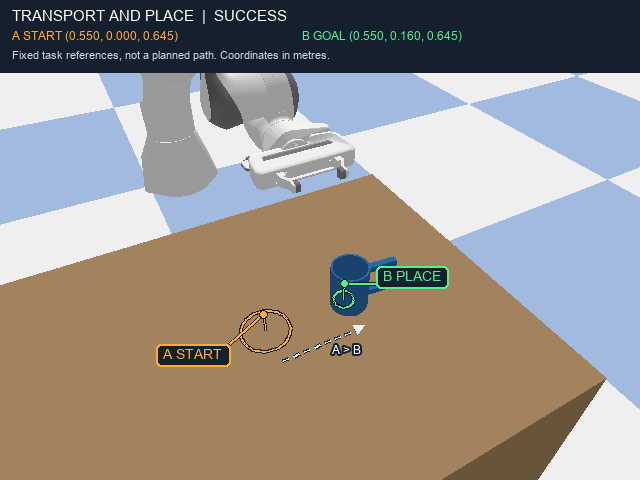
\includegraphics[width=0.24\linewidth]{figures/task_transport.png}\hfill
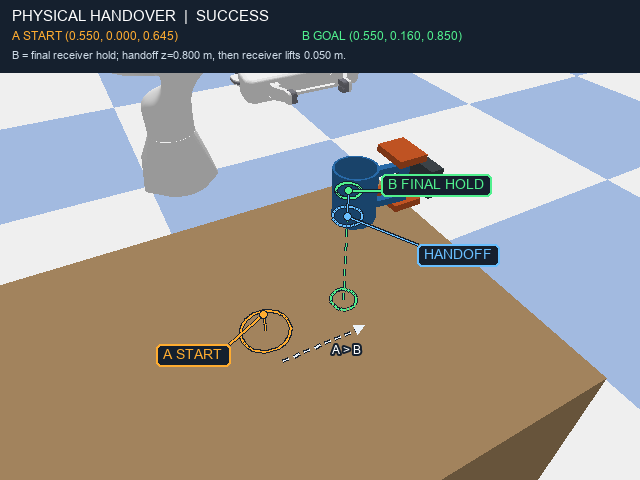
\includegraphics[width=0.24\linewidth]{figures/task_handover.png}\hfill
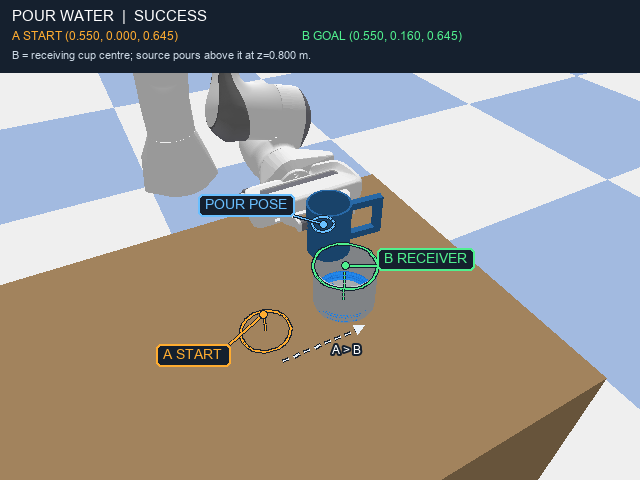
\includegraphics[width=0.24\linewidth]{figures/task_pour.png}
\caption{The three complete tasks in PyBullet: transport and placement (left), cooperative handover to a receiving gripper (centre), and PBF pouring into a receiving cup (right). Final frames of seed-0 demonstrations that used an earlier candidate set; they illustrate the controllers and are not benchmark episodes.}
\label{fig:tasks}
\end{figure}

Figure~\ref{fig:tasks} shows the three sequences. All tasks require no disallowed collisions or drops, and terminal uprightness within $5^\circ$, linear speed at most 0.02 m/s, and angular speed at most $5^\circ$/s throughout the 1 s terminal window. A pickup followed by a failed release, transfer, tilt, or retreat counts as failure.

\section{Candidate generation and selectors}
\subsection{Candidate families and analytical baselines}
M0--M2, M4, and M5 are analytical or empirical baselines; Section~\ref{sec:llm} describes language-based M3, its ablation A1, and rule-only M6.

We deterministically sample 116 mug-local poses (\code{multifamily\_v3p}) across four families: handle, rim, top-down body (top), and side body (side). Rim and handle grasps remain selectable outside the ideal cylindrical-body contact model; their zero geometry-score placeholder means \emph{unmodeled}, not zero success probability.

\textbf{M0} produces a seeded random ranking. We also report the exact uniform expectation by averaging all feasible candidate outcomes per scene; one random realization is not its expectation.

\textbf{M1}, the benchmark's \code{static\_load\_margin\_v2}, scores a supported body grasp as
\begin{equation}
S_1(g)=\frac{1}{1+L_0(g)+E(g)},\qquad
E(g)=\frac{h_p}{m_e(g)+h_p},
\end{equation}
where $L_0$ is normalized static force demand, $h_p=8$ mm is assumed pad half-height, and $m_e$ is the remaining contact-edge margin. The demand proxy resolves force into closing-axis and tangential components, and moment into torsion and bending:
\begin{equation}
N_{\rm req}=\frac{|F_n|}{2}+\frac{\|F_t\|}{2\mu}
+\frac{\|\tau_b\|}{2\mu r}+\frac{|\tau_n|}{2\mu r_\tau},\qquad
L_0(g)=\frac{N_{\rm req}}{N_{\rm cap}}.
\end{equation}
Here $r$ is body radius, $\mu=0.6$, $r_\tau=8$ mm, and $N_{\rm cap}=15$ N per finger. These are declared surrogate assumptions, not measured forces or calibrated simulator coefficients. Section~\ref{sec:wrench} uses a distinct wrench formulation; its scores do not enter Table~\ref{tab:main}.

\textbf{M2} extends this model to $S_2(g,t)=[1+R(g,t)]^{-1}$. Transport risk uses the maximum estimated load ratio along nominal motion plus the edge penalty. Handover additionally penalizes handle occlusion, receiver swept-volume overlap, inaccessible handle volume, withdrawal toward the receiver, and small clearance. Pouring adds rim/handle obstruction and clearance terms. Motion loads smoothly approximate commanded stages, not measured future accelerations; liquid is a fixed lumped mass without drainage or slosh. M1/M2 rank supported body candidates first and append unsupported candidates in ID order, introducing a family-coverage bias.

\textbf{M4} orders families by empirical task success on training seeds 0--9, then static quality where supported and ID. Pouring uses PBF training outcomes for the PBF-table comparison.

\textbf{M5} first prefers a fixed task-specific part (handle for placement/pouring, body for handover), then ranks by $Q(g)-d(g,p_t)/(0.05\,\mathrm m)$, where $Q$ is static quality and $p_t$ the preferred part centre. Unsupported quality uses the mean supported score. No handle candidate passes the pouring filter, so fallback ordering matters. M5 is an engineering surrogate, not a published method reproduced end to end.

\subsection{Language prompts, ablation, and rule-only control}
\label{sec:llm}
We evaluate two recorded language-model configurations: \code{gpt-5.6-luna} through the Codex adapter with low reasoning effort (GPT in the tables), and \code{gemini-3.8-flash} through the Gemini adapter with low thinking level (Gemini). M3 includes the task ID and intention; A1 removes them while retaining the version-specific system prompt and task-filtered candidates. A1 removes explicit task text, not every indirect task cue.

Three prompt versions change the input contract. \textbf{v1} calls geometry score a higher-is-better prior without explaining unsupported zeros. \textbf{Mechanics} (\code{v2\_physics}) clarifies zero as unscored, corrects the overly broad opening-obstruction label, and supplies motion/clearance constraints without naming a preferred grasp family. \textbf{Preferences} (\code{v2}) explicitly prioritizes outer-handle or suitable rim grasps for placement, top-down rim grasps for handover, and high-scoring top body grasps for pouring. These versions change several instructions together; they are not an isolated causal test of score clarification or spatial reasoning.

Responses must contain a valid selected ID and a complete, duplicate-free permutation with that ID first. One format-repair attempt is permitted; persistent invalid output uses a deterministic geometry-based fallback. Repair messages contain validation errors, not execution outcomes. \textbf{M6} implements the v2 preference tiers directly from public fields, breaking ties by score and ID, without a model call. The preferences and M6 were developed after evaluation outcomes were inspected. They are retrospective controls, not independently validated policies.

\subsection{Task-conditioned wrench-space evaluation}
\label{sec:wrench}
Static and task-risk surrogates use body-contact proxies, leaving rim and handle grasps unmodeled. Our extension evaluates finite task-required wrenches through predicted contacts, linearized friction cones, and shared finger capacities. Strict equilibrium minimizes worst utilization; relaxed optimization minimizes worst scaled residual under capacity bounds, then utilization within that checked residual bound plus slack (Appendix~\ref{app:wrench}). Neither establishes complete-task success: contact simultaneity, collisions, tracking, release, receiver access, and liquid transfer remain outside this numerical guarantee. We examine these uncalibrated formulations through numerical consistency and contact-model checks. The main archived benchmark evaluates complete-task selection using surrogate rankings, without comparing the wrench-space methods with language-based selectors.

\section{Experimental design}
The main comparison uses R3 archived executions for placement/handover and the corresponding full PBF pouring table. Seeds 0--9 train M4; seeds 10--29 supply 20 evaluation scenes per task. Those scenes had already appeared in development analysis, so we call them \emph{evaluation seeds}, not a blind test set. Two models, three prompts, and M3/A1 yield 12 configurations and 720 selection trials. There is one initial response per configuration--task--seed, with repair permitted; this does not estimate repeated-model variability. Of the 720 trials, 712 had valid initial responses, eight needed a repair attempt, and two of those used the geometry fallback; all final selections are valid, and success includes fallback behavior. Gemini records store one constant latency value, so the logs do not support provider cost or speed comparisons.

We score selected IDs by lookup into the same task/seed execution tables. All 458 feasible pouring candidates across 30 seeds have a PBF outcome, enabling both a uniform expectation and an oracle. The oracle, which succeeds whenever any feasible candidate succeeds, is an outcome-aware upper bound, not an executable baseline. A separate local PBF rerun of 98 distinct selected seed--candidate pairs is a reproducibility check, not additional scenes.

The primary endpoint is per-task binary success over evaluation seeds. Physical failures remain in the denominator; missing outcomes, numerical errors, and call failures must be reported separately. All entries in Table~\ref{tab:main} have 20 scored trials. The three-task sum counts 60 task--seed outcomes descriptively; shared seeds and fixed tasks preclude treating it as 60 independent draws for inference.

We use per-task 95\% Wilson intervals with scenes as units. Paired comparisons use a two-sided exact sign/McNemar test on discordant seeds. We retain the archived Holm adjustment over all 170 valid comparisons, including proxy and rerun endpoints; the added M6 control is descriptive and does not change this historical family. Tests are exploratory because scenes and prompts were reused.

\section{Results and analysis}
\subsection{Complete-task success and grasp-family effects}
\begin{table}[t]
\caption{Success counts on seeds 10--29; every task entry is out of 20. Pouring uses the full archived PBF table, not the proxy or local rerun. The total is descriptive, out of 60. M3 has task text; A1 omits it. Pref. and M6 contain retrospective explicit preferences.}
\label{tab:main}
\centering\footnotesize
\begin{tabular}{lrrrr}
\toprule
Method & Place & Handover & Pour (PBF) & Total \\
\midrule
M0 Random & 15 & 11 & 16 & 42 \\
M1 Static v2 & 17 & 5 & 13 & 35 \\
M2 Task risk & 19 & 11 & 15 & 45 \\
M4 Family prior & 18 & 17 & 12 & 47 \\
M5 Part surrogate & 20 & 5 & 13 & 38 \\
\midrule
GPT v1 M3 & 15 & 4 & 13 & 32 \\
GPT v1 A1 & 17 & 5 & 13 & 35 \\
GPT Mech. M3 & 9 & 5 & 11 & 25 \\
GPT Mech. A1 & 10 & 2 & 12 & 24 \\
GPT Pref. M3 & 18 & 20 & 16 & 54 \\
GPT Pref. A1 & 16 & 6 & 9 & 31 \\
\midrule
Gemini v1 M3 & 19 & 5 & 14 & 38 \\
Gemini v1 A1 & 9 & 1 & 14 & 24 \\
Gemini Mech. M3 & 10 & 20 & 13 & 43 \\
Gemini Mech. A1 & 13 & 9 & 8 & 30 \\
Gemini Pref. M3 & 19 & 20 & 16 & 55 \\
Gemini Pref. A1 & 18 & 4 & 11 & 33 \\
\midrule
M6 Prompt rules & 18 & 20 & 16 & 54 \\
Uniform expected count & 15.9 & 10.4 & 12.3 & 38.6 \\
Oracle upper bound & 20 & 20 & 20 & 60 \\
\bottomrule
\end{tabular}

\end{table}

Table~\ref{tab:main} shows substantial task dependence. M5 places all 20 mugs successfully but completes only five handovers. M4 improves handover to 17/20 but obtains 12/20 in PBF pouring. M2 reaches 19/20 placement yet only 11/20 handover.

\begin{figure}[t]
\centering
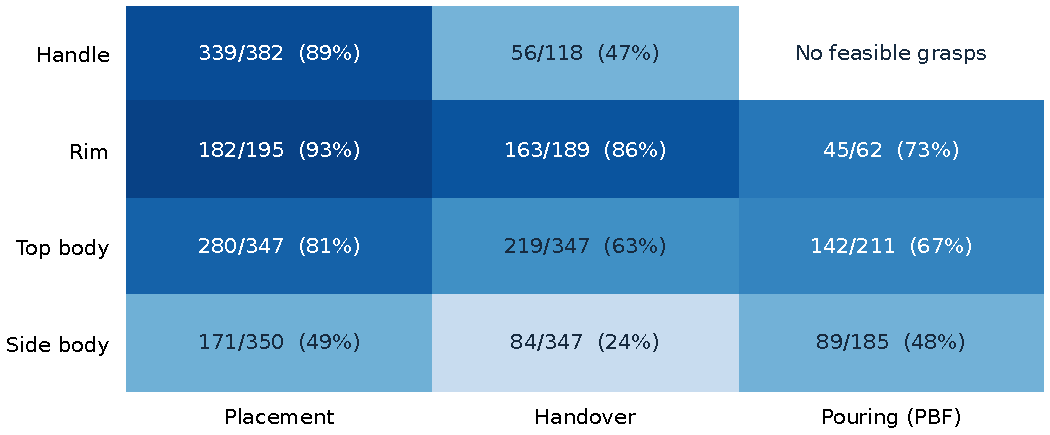
\includegraphics[width=0.56\linewidth]{figures/family_task.pdf}
\caption{Pooled R3 execution outcomes across seeds 0--29, grouped by family. Labels show successes/executions and rounded percentages. These correlated candidate outcomes describe the feasible pool, not selector performance. Handle pouring is unavailable because no handle candidate passes the filter.}
\label{fig:family}
\end{figure}

Figure~\ref{fig:family} separates the pool from the selector: rim grasps complete 86\% of handovers versus 24\% for side grasps, while PBF pouring is less separated (rim 73\%, top 67\%, side 48\%). The feasible pool thus contains task signal that static scores fail to exploit. The oracle succeeds in every evaluation scene for all three tasks, so candidate coverage does not force failure in these scenes.

GPT and Gemini with preferences score 54/60 and 55/60. However, M6 scores 54/60, including the same 20/20 handovers and 16/20 PBF pours. Both v2 models select top-family grasps for every pour and rim-family grasps for every handover. This supports the usefulness of supplied preferences, but does not establish an advantage from model reasoning. Their 16/20 PBF pours only tie realized M0.

\subsection{What the prompt ablations establish}
Across 240 v1 selections (two models, M3/A1, three tasks), neither model selects a rim or handle grasp. This is consistent with ambiguous zero scores and misleading tags steering selection toward modeled body grasps. Because several instructions change together, neither issue is isolated as the cause.

With mechanics prompts, Gemini M3 selects rim grasps for all handovers and improves from 5/20 to 20/20. Against v1 it has 15 paired wins and no losses, exact $p=6.10\times10^{-5}$ and archived Holm $p=0.0103$. Against mechanics A1 (9/20), it has 11 wins and no losses: exact $p=9.77\times10^{-4}$, but Holm $p=0.1563$, which does not pass a 0.05 familywise threshold. The change is compatible with useful task-conditioned selection, without proving general spatial reasoning.

GPT mechanics reaches 5/20 handovers versus A1's 2/20; raw paired outcomes are three wins, zero losses, and $p=0.25$. Its 25/60 total shows that the clarified interface does not reliably help both configurations. GPT/Gemini preference prompts outperform their A1 variants in handover (20 versus 6 and 4), with adjusted $p=0.0200$ and $0.00519$. These differences include explicit recommendations, not merely access to a task name. No method's improvement over M0 survives the archived Holm correction on the three primary endpoints. Perfect observed performance remains uncertain: 20/20 has Wilson interval [0.839, 1.000], and 16/20 has [0.584, 0.919].

\subsection{Pouring metric and reproducibility sensitivity}
The \code{proxy\_margin} mode checks spout trajectory and conservative clearances without particles. Across the 458 R3 feasible pouring executions, its result agrees with PBF in 347 cases (75.8\%). A geometric criterion therefore cannot substitute for the liquid endpoint.

\begin{table}[htbp]
\caption{Pouring sensitivity on the same 20 evaluation seeds. R3 full PBF is primary; local PBF re-executes selected candidates. R4 changes the wrist--hand collision setting and is a separate sensitivity condition. Counts are out of 20; -- means not evaluated here.}
\label{tab:sensitivity}
\centering\footnotesize
\begin{tabular}{lrrrr}
\toprule
Method & R3 proxy & R3 PBF & Local PBF & R4 PBF \\
\midrule
M0 Random & 13 & 16 & 16 & 16 \\
M1 Static v2 & 12 & 13 & 15 & 17 \\
M2 Task risk & 13 & 15 & 15 & 18 \\
M4 Family prior & 14 & 12 & 13 & 12 \\
M5 Part surrogate & 12 & 13 & 15 & 17 \\
GPT Pref. M3 & 18 & 16 & 17 & -- \\
Gemini Pref. M3 & 18 & 16 & 17 & -- \\
\bottomrule
\end{tabular}

\end{table}

GPT/Gemini preference prompts obtain 18/20 proxy but 16/20 archived PBF pours (Table~\ref{tab:sensitivity}). M0 rises from 13/20 to 16/20, eliminating the apparent pouring advantage.

Local PBF gives 17/20 for both preference models, versus 16/20 archived; M1 changes from 13/20 to 15/20. Historical tables lack complete environment fingerprints, so cross-machine reproducibility is not established.

\subsection{Simulator artifact and corrected-scene analysis}
A later audit found persistent self-contact between Panda link7 and the hand, separated in the URDF by a fixed joint. In R3 this impeded large wrist rotations and disproportionately affected side approaches. R4 (\code{wide\_strict\_v3}) disables only this collision pair while preserving candidates and scene seeds. Across the three-task proxy archive, pregrasp timeouts decrease from 222 to two. Pooled side success improves from approximately 49\% to 63\% for placement, 24\% to 31\% for handover, and 48\% to 66\% for PBF pouring.

On R4 evaluation seeds, M0 achieves 19/20 placement, 14/20 handover, and 16/20 PBF pouring; M2 achieves 18/20, 5/20, and 18/20. R4 M6 obtains 19/20, 20/20, and 18/20. The complete 12-configuration language benchmark was collected against R3; we do not relabel it as R4 or mix it with corrected-scene scores. Because the artifact mainly affected side approaches, R3 alone cannot show that its family differences arise solely from physical task requirements.

\section{Discussion, limitations, and reproducibility}
\label{sec:discussion}
Release clearance, receiver access, and trajectory reachability go beyond static contact margins or part names. Direct rules match the strongest prompt-conditioned outcomes and are a necessary reference before attributing gains to language.

Limitations include one mug and donor/receiver design, synthetic pose noise, fixed trajectories, one model sample per condition, reused scenes, and simulator artifacts. Information access differs and preference prompts are outcome informed. Unseen shapes, human motion, visual occlusion, and hardware execution remain untested. The wrench-space ranker uses uncalibrated contact and force models and has not been evaluated on the evaluation seeds.

A stronger experiment would freeze labels, scores, prompts, and M6 before fresh seeds (e.g., 30--49), use the corrected collisions, repeat model sampling, and vary mug geometry; useful features include wrist rotation demand, joint-limit margins, and receiver swept-volume clearance.

\paragraph{Reproducibility.}
The public repository (linked in the abstract) archives candidates, filters, episodes, selected IDs, and messages; its README gives run instructions. \path{prepare_results.py} re-checks per-seed counts, selected episodes, paired tests, and the Holm adjustment, evaluates M6, and regenerates the benchmark tables and pooled-family figure without new physics or model calls; the report README maps each result to its source directory.

\paragraph{Team contributions.}
\textbf{Xie Lin (Part A, simulation)} built the PyBullet scenes, staged controllers, and terminal evaluator, including PBF pouring; the execution-consistent feasibility filter; and the R3/R4 execution archives, including the collision-artifact correction. \textbf{Zhang Yijie (Part B, grasps and baselines)} built the grasp candidate generator and geometric features; the analytical baselines, including the static and task-risk scores; and the exploratory wrench-space scoring extension. \textbf{Yao Xiaolu (Part C, language-model evaluation)} built the language-model selector interface and prompt versions; the 720-trial multi-model evaluation with its output audit; and the paired statistical analysis and report draft.

\section{Conclusion}
Task-aware grasp selection requires evaluating what happens after pickup. Our mug benchmark exposes task-dependent families, but prompt preferences, missing-value semantics, pouring metrics, and simulator artifacts can dominate measured improvements: explicit-preference models reach 90.0\% and 91.7\% three-task success, and direct rules 90.0\%. The defensible outcome is an auditable framework and a bounded empirical diagnosis, not a general advantage of language-model grasp selection.

% References and the technical appendix are excluded from the confirmed main-paper limit.
\clearpage
\begin{thebibliography}{9}
\bibitem[Dang and Allen(2012)]{dang2012}
Hao Dang and Peter K. Allen.
Semantic grasping: Planning robotic grasps functionally suitable for an object manipulation task.
In \emph{IEEE/RSJ International Conference on Intelligent Robots and Systems}, pp. 1311--1317, 2012.
\url{https://www.cs.columbia.edu/~allen/PAPERS/dang_iros_2012.pdf}.

\bibitem[Murali et al.(2021)]{murali2021}
Adithyavairavan Murali, Weiyu Liu, Kenneth Marino, Sonia Chernova, and Abhinav Gupta.
Same object, different grasps: Data and semantic knowledge for task-oriented grasping.
In \emph{Proceedings of the 2020 Conference on Robot Learning}, PMLR 155:1540--1557, 2021.
\url{https://proceedings.mlr.press/v155/murali21a.html}.

\bibitem[Ferrari and Canny(1992)]{ferrari1992}
Carlo Ferrari and John Canny.
Planning optimal grasps.
In \emph{Proceedings of the IEEE International Conference on Robotics and Automation}, vol.~3, pp. 2290--2295, 1992.
\url{https://doi.org/10.1109/ROBOT.1992.219918}.

\bibitem[Mahler et al.(2017)]{mahler2017}
Jeffrey Mahler, Jacky Liang, Sherdil Niyaz, Michael Laskey, Richard Doan, Xinyu Liu, Juan Aparicio, and Ken Goldberg.
Dex-Net 2.0: Deep learning to plan robust grasps with synthetic point clouds and analytic grasp metrics.
In \emph{Robotics: Science and Systems XIII}, 2017.
\url{https://doi.org/10.15607/RSS.2017.XIII.058}.

\bibitem[Tang et al.(2023)]{tang2023}
Chao Tang, Dehao Huang, Wenqi Ge, Weiyu Liu, and Hong Zhang.
GraspGPT: Leveraging semantic knowledge from a large language model for task-oriented grasping.
\emph{IEEE Robotics and Automation Letters}, 8(11):7551--7558, 2023.
\url{https://arxiv.org/abs/2307.13204}.

\bibitem[Ichter et al.(2023)]{ichter2023}
Brian Ichter, Anthony Brohan, Yevgen Chebotar, Chelsea Finn, Karol Hausman, et al.
Do as I can, not as I say: Grounding language in robotic affordances.
In \emph{Proceedings of the 6th Conference on Robot Learning}, PMLR 205:287--318, 2023.
\url{https://proceedings.mlr.press/v205/ichter23a.html}.

\bibitem[Macklin and M\"uller(2013)]{macklin2013}
Miles Macklin and Matthias M\"uller.
Position based fluids.
\emph{ACM Transactions on Graphics}, 32(4), Article 104, 2013.
\url{https://mmacklin.com/pbf_sig_preprint.pdf}.

\bibitem[Coumans and Bai(2016--2021)]{bullet}
Erwin Coumans and Yunfei Bai.
PyBullet, a Python module for physics simulation for games, robotics and machine learning.
2016--2021.
\url{http://pybullet.org}.
\bibitem[Appius et al.(2025)]{appius2025}
Aurel X. Appius, \'Emiland Garrab\'e, Fran\c{c}ois H\'el\'enon, Mahdi Khoramshahi, Mohamed Chetouani, and St\'ephane Doncieux.
Task-Aware Robotic Grasping by evaluating Quality Diversity Solutions through Foundation Models.
In \emph{2025 IEEE/RSJ International Conference on Intelligent Robots and Systems (IROS)}, pp. 1035--1040, 2025.
\url{https://doi.org/10.1109/IROS60139.2025.11246636}. Preprint: \url{https://arxiv.org/abs/2411.14917}.

\end{thebibliography}

\clearpage
\appendix
\numberwithin{equation}{section}
\section{Task-Conditioned Wrench-Space Formulation}
\label{app:wrench}
This appendix specifies the implemented evaluation extension in Section~\ref{sec:wrench}, independently of the benchmark's surrogate M1/M2. The distinct method identifiers are \path{m1_gws_v2}, \path{m2_gws_trajectory_v2}, \path{relaxed_m1_task_lex_v1}, and \path{relaxed_m2_task_lex_v1}.

\subsection{Contact wrench map and linearized friction}
For contact $i$, let $p_i$ be its predicted position, $n_i$ its outward unit normal, and $o$ the common wrench reference point, all in mug coordinates. Let $d_i=-n_i$ and let $t_{i1},t_{i2}$ be the deterministic orthonormal tangents constructed by the implementation. With friction coefficient $\mu_i\ge0$, the polyhedral cone generators are
\begin{equation}
\theta_j=\frac{2\pi j}{k},\qquad
v_{ij}=d_i+\mu_i\bigl(t_{i1}\cos\theta_j+t_{i2}\sin\theta_j\bigr),
\quad j=0,\ldots,k-1.
\label{eq:cone}
\end{equation}
The supported direction counts $k\in\{8,16,32\}$ use nested samples of one 32-angle grid. For $\mu_i=0$, the implementation retains only $d_i$. Each generator has unit inward normal component, not unit Euclidean norm; its nonnegative coefficient $\lambda_{ij}$ is therefore a normal-force contribution in newtons. The point-contact wrench map is
\begin{equation}
  a_{ij}=\begin{bmatrix}v_{ij}\\(p_i-o)\times v_{ij}\end{bmatrix},\qquad
 A=[\,a_{ij}\,]_{i,j},\qquad w_{\rm contact}=A\lambda,\quad\lambda\ge0.
\label{eq:wrench-map}
\end{equation}
The top three rows are forces (N), and the bottom three are moments (N\,m). No independent torsional moment is added at a contact. Multiple points per finger assume simultaneous, independent load-bearing contacts.

\subsection{Shared capacity and finite task demands}
Let $I_f$ contain the modeled contacts assigned to finger capacity group $f$, with declared capacity $b_f$ (N). Shared capacity requires
\begin{equation}
 \sum_{i\in I_f}\sum_j\lambda_{ij}\le b_f\quad\text{for every }f,
 \qquad B\lambda\le b.
\label{eq:capacity}
\end{equation}
The development settings are $\mu_i=0.5$, $k=16$, and $b_f=5$ N per finger, distinct from the benchmark surrogate assumptions. Each group row of $B$ has a one for every generator assigned to that group and zero elsewhere. Explicitly supplied local contact limits add rows to $B,b$; unspecified local limits add none. Additional points or cone directions do not grant extra finger capacity.

For task $t$ and candidate $g$, the input is a finite required-contact-wrench set
\begin{equation}
 \mathcal W_{t,g}=\{w_s\in\mathbb R^6:s=1,\ldots,K\}.
\label{eq:demands}
\end{equation}
Quasi-static evaluation uses a common declared task-wrench set across candidates; trajectory evaluation may use candidate-dependent predicted motion and inertial loads. Required contact wrench balances external loads (the negative external wrench in static equilibrium). All forces and moments use the same mug frame and reference $o$. Only the declared donor-supported motion scope is modeled: unknown support allocation and missing required loads cannot silently become zero demands. Trajectory liquid loads use the declared rigid/lumped approximation, not simulated drainage or sloshing. Bitwise-identical demands may share a computational block, while every original required scenario and its residual are retained and checked.

\subsection{Strict equilibrium and worst utilization}
For each required $w_s$, the strict LP is
\begin{equation}
 \begin{aligned}
 u_s^*=\min_{\lambda_s,u_s}\;&u_s\\
 \text{subject to }&A\lambda_s=w_s,\quad B\lambda_s\le u_s b,\\
 &\lambda_s\ge0,\quad u_s\ge0.
 \end{aligned}
\label{eq:strict}
\end{equation}
There is deliberately no upper bound $u_s\le1$. A finite solution with $u_s>1$ expresses excess demand relative to the declared capacity; it is distinct from an equilibrium that cannot be represented at any capacity scaling. Only if every required scenario has a checked optimal result is the task score defined as
\begin{equation}
 \rho=\max_s u_s^*,\qquad Q_{\rm strict}=1-\rho.
\label{eq:strict-score}
\end{equation}
A negative score is retained. No partial maximum substitutes for a complete task score. Exact equilibrium is the mathematical constraint; the solver's floating-point witness is checked in physical units against explicit tolerances. Optional positive row scaling changes numerical conditioning, not the required wrench or feasible set. Strict ranking orders scored candidates by increasing $\rho$, then ID.

\subsection{Relaxed task-level two-stage optimization}
The relaxed solver uses common, explicit scales $F_*>0$ (N) and $L>0$ (m):
\begin{equation}
 S=\operatorname{diag}\!\left(\frac1{F_*},\frac1{F_*},\frac1{F_*},
 \frac1{F_*L},\frac1{F_*L},\frac1{F_*L}\right),\qquad
 r_s=\|S(A\lambda_s-w_s)\|_\infty.
\label{eq:scale}
\end{equation}
The residual is dimensionless and does not equate force error with torque error in unscaled SI units. Stage 1 includes all required demands in one LP with one shared residual objective:
\begin{equation}
 \begin{aligned}
 R^*=\min_{\{\lambda_s\},R}\;&R\\
 \text{subject to }&-R\mathbf1\le S(A\lambda_s-w_s)\le R\mathbf1,\quad s=1,\ldots,K,\\
 &B\lambda_s\le b,\quad\lambda_s\ge0\quad(s=1,\ldots,K),\qquad R\ge0.
 \end{aligned}
\label{eq:relaxed-one}
\end{equation}
There is one force vector per demand, with the same per-finger bounds at each demand; capacities are not summed across time. In floating-point execution, the recorded risk $\widehat R$ is the checked objective upper bound, namely the maximum of the returned $R$ and the independently recomputed worst residual. Stage 2 fixes
\begin{equation}
 \delta=\delta_{\rm abs}+\delta_{\rm rel}|\widehat R|,\qquad \varepsilon=\widehat R+\delta,
\label{eq:radius}
\end{equation}
then solves one shared-utilization LP:
\begin{equation}
 \begin{aligned}
 u^*=\min_{\{\lambda_s\},u}\;&u\\
 \text{subject to }&-\varepsilon\mathbf1\le S(A\lambda_s-w_s)\le\varepsilon\mathbf1,
                       \quad s=1,\ldots,K,\\
 &B\lambda_s\le u b,\quad\lambda_s\ge0\quad(s=1,\ldots,K),\qquad 0\le u\le1.
 \end{aligned}
\label{eq:relaxed-two}
\end{equation}
The development scales are $F_*=1$ N and $L=0.1$ m; the configured slack defaults are $\delta_{\rm abs}=10^{-7}$ and $\delta_{\rm rel}=0$. The recorded utilization $\widehat u$ is the checked upper bound: the maximum of the returned $u$ and reconstructed capacity ratios for positive entries of $b$. Zero-capacity rows are checked directly. Independent per-scenario lexicographic minimization would define a different method.

\subsection{Numerical statuses, ranking, and interpretation}
Strict solver outcomes distinguish \path{optimal}, \path{infeasible}, missing parameters/dependencies, invalid input, and numerical failure. At task level, an unscored demand prevents a complete strict score. Relaxed results receive \path{scored_conditional} only when both stages pass original-matrix primal, dual, and objective-gap checks; numerical errors and missing parameters remain explicit, rather than becoming physical failures. Geometry-invalid contacts remain separately unscored. The Stage-2 realized residual, the Stage-1 objective, and numerical constraint violations are different quantities. A positive relaxed residual is permitted by design and is not an exact-equilibrium certificate.

Relaxed ranking minimizes $(\widehat R,\widehat u)$ using anchored numerical bands. For either objective $z$, the lowest remaining value $a$ anchors a band
\begin{equation}
 z\le a+\eta_{\rm abs}+\eta_{\rm rel}\max(1,|a|).
\label{eq:bands}
\end{equation}
Residual bands are formed first, then utilization bands within each residual band; IDs resolve ties within the second band. Defaults are $\eta_{\rm abs}=10^{-6}$ for each objective and $\eta_{\rm rel}=10^{-8}$. Bands are anchored, not chained through pairwise near-ties. Unscored IDs appear only in a diagnostic tail; if no candidate has a complete score, the selector abstains. Neither near-ties nor complete scores establish force closure or physical success probability.

\end{document}
